% --- UNIVERSAL PREAMBLE BLOCK ---
\documentclass[11pt, a4paper]{article}
\usepackage[a4paper, top=2.5cm, bottom=2.5cm, left=2cm, right=2cm]{geometry}
\usepackage[T1]{fontenc}
\usepackage[utf8]{inputenc}
\usepackage{lmodern}
\usepackage{amsmath}
\usepackage{array}
\usepackage{booktabs}
\usepackage{xcolor}
\usepackage{verbatim}
\usepackage{graphicx}
\graphicspath{{./}{../../graficos/}}
\usepackage{fancyhdr}
\usepackage{titlesec}
\usepackage{lastpage}
\usepackage[section]{placeins}
\usepackage[hidelinks]{hyperref}

\usepackage[spanish, es-tabla]{babel}

% Add because main language is not English
\usepackage{enumitem}
\setlist[itemize]{label=-}

% Professional Color Palette for Chaco For Ever (Gray/Teal/Red/Amber)
\definecolor{primary}{HTML}{0F172A}    % Dark Slate
\definecolor{alertred}{HTML}{DC2626}   % Red-600
\definecolor{accentgreen}{HTML}{0F766E}% Teal-700
\definecolor{warnamber}{HTML}{D97706}  % Amber-600
\definecolor{lightgray}{HTML}{F8FAFC}  % Slate-50
\definecolor{bordergray}{HTML}{E2E8F0} % Slate-200
\definecolor{darkgray}{HTML}{475569}   % Slate-600

% Custom styled frame box command for warnings
\newcommand{\alertbox}[2]{%
  \noindent\colorbox{lightgray}{%
    \parbox{\dimexpr\textwidth-2\fboxsep\relax}{%
      \raggedright
      \smallskip
      \textbf{\color{alertred}{#1}}\par\smallskip
      \small #2\par\smallskip
    }%
  }%
  \par\vspace{3mm}
}

% Custom command for green highlighting
\newcommand{\successbox}[2]{%
  \noindent\colorbox{lightgray}{%
    \parbox{\dimexpr\textwidth-2\fboxsep\relax}{%
      \raggedright
      \smallskip
      \textbf{\color{accentgreen}{#1}}\par\smallskip
      \small #2\par\smallskip
    }%
  }%
  \par\vspace{3mm}
}

% Colores de resaltado tipo marcador (highlighter)
\definecolor{markred}{HTML}{FEE2E2}    % rojo claro — dato negativo
\definecolor{markgreen}{HTML}{D1FAE5}  % verde claro — dato positivo
\definecolor{markamber}{HTML}{FEF3C7}  % ámbar claro — dato clave neutro

% Resaltados en línea (fondo tenue + negrita)
\newcommand{\mR}[1]{\textbf{#1}}
\newcommand{\mG}[1]{\textbf{#1}}
\newcommand{\mA}[1]{\textbf{#1}}

% Etiqueta para marcar informacion que NO sale del partido en si
\newcommand{\previa}{{\footnotesize\textbf{\color{warnamber}[PREVIA]}}\ }
\newcommand{\temp}{{\footnotesize\textbf{\color{darkgray}[TEMPORADA]}}\ }

% Caja neutra para resumenes de DATOS objetivos (header slate, sin carga editorial)
\newcommand{\databox}[2]{%
  \noindent\colorbox{lightgray}{%
    \parbox{\dimexpr\textwidth-2\fboxsep\relax}{%
      \raggedright
      \smallskip
      \textbf{\color{primary}{#1}}\par\smallskip
      \small #2\par\smallskip
    }%
  }%
  \par\vspace{3mm}
}

\setlength{\parindent}{0pt}
\setlength{\parskip}{6pt}

% --- Encabezado / pie de página ---
\pagestyle{fancy}
\fancyhf{}
\renewcommand{\headrulewidth}{0.4pt}
\renewcommand{\footrulewidth}{0.4pt}
\fancyhead[L]{\small\color{darkgray}\textsc{Chaco For Ever} $\bullet$ Informe de Partido}
\fancyhead[R]{\small\color{darkgray}Fecha 20 $\bullet$ 2026}
\fancyfoot[L]{\footnotesize\color{darkgray}Uso interno del Cuerpo Técnico}
\fancyfoot[R]{\footnotesize\color{darkgray}Página \thepage\ de \pageref{LastPage}}

% --- Estilo de secciones (regla de color debajo del título) ---
\titleformat{\section}
  {\normalfont\Large\bfseries\color{primary}}
  {\thesection}{0.6em}{}
  [\vspace{-2mm}\noindent{\color{accentgreen}\rule{\textwidth}{1.2pt}}]
\titlespacing*{\section}{0pt}{4mm}{4mm}

\titleformat{\subsection}
  {\normalfont\large\bfseries\color{darkgray}}
  {\thesubsection}{0.6em}{}
\titlespacing*{\subsection}{0pt}{3mm}{2mm}

\hypersetup{
  pdftitle={Informe de Partido -- Chaco For Ever vs San Telmo 2026},
  pdfauthor={Departamento de Big Data \& Análisis Táctico},
  pdfsubject={Fecha 20 -- Primera Nacional 2026},
}

\begin{document}

% --- HEADER BLOCK ---
\begin{center}
  \colorbox{primary}{%
    \parbox{\dimexpr\textwidth-2\fboxsep\relax}{%
      \vspace{4mm}
      \centering
      \color{white}
      \textsc{\Large Chaco For Ever} \\
      \smallskip
      \textbf{\Large INFORME DE PARTIDO} \\
      \vspace{1mm}
      \small Fecha 20 $\bullet$ San Telmo 1 -- 3 Chaco For Ever $\bullet$ Primera Nacional 2026
      \vspace{4mm}
    }%
  }
\end{center}

\vspace{4mm}

% --- METADATA ---
\begin{tabular}{ll}
  \textbf{Destinatarios:} & Cuerpo Técnico, Comisión Directiva \\
  \textbf{Creadores:} & Cordeiro Mariano Angel y Casco Tobias \\
  \textbf{Contacto:} & cordeiromariano17@gmail.com \\
  \textbf{Partido:} & San Telmo 1 -- 3 Chaco For Ever (de visitante, entretiempo 0-2) \\
  \textbf{Goles:} & Romero (9'), Gaggi (38'), Romero (89', penal) \quad / \quad Motroni (46') \\
  \textbf{Alcance del Análisis:} & Fecha 20, leída con las herramientas de la temporada 2026 \\
\end{tabular}

\vspace{3mm}
\noindent\colorbox{lightgray}{%
  \parbox{\dimexpr\textwidth-2\fboxsep\relax}{%
    \smallskip
    \small Este informe primero presenta los \textbf{datos del partido con objetividad} (secciones 1 a 4) y
    deja la \textbf{interpretación y nuestro punto de vista para el final} (sección 5, ``Nuestra Lectura'').
    Además, cuando usamos algo del \textbf{\color{warnamber}informe pre-partido} lo marcamos con \previa, y
    cuando usamos un dato de la \textbf{\color{darkgray}temporada} (fuera de este partido) lo marcamos con
    \temp. Así queda claro qué es dato del partido, qué es contexto de afuera y qué es opinión nuestra.\smallskip
  }%
}
\vspace{2mm}
\hrule
\vspace{4mm}

% ==================================================================
% BLOQUE OBJETIVO (Secciones 1-4): solo datos, sin interpretacion
% ==================================================================

% --- SECCIÓN 1: QUÉ PASÓ EN EL PARTIDO ---
\section*{1. El Resultado y los Números}

San Telmo 1 -- 3 Chaco For Ever, de visitante. Al entretiempo, 0-2. La secuencia de goles fue: Romero al 9' (asistencia de L. Fernández), Gaggi al 38' (asistencia de Romero), Motroni descontó para San Telmo al 46' (asistencia de Iritier) y Romero cerró de penal al 89'.

En el informe vas a ver la sigla \textbf{xG}. Es una forma sencilla de medir qué tan clara fue una situación de gol: un valor cercano a 1 es un gol casi hecho, y uno cercano a 0 es un remate muy difícil. Sumando el xG de un equipo se ve cuánto peligro generó en total, más allá de si la embocó o no.

\begin{table}[h!]
  \centering
  \caption{Números del partido (Chaco / San Telmo)}
  \vspace{2mm}
  \begin{tabular}{lll}
    \toprule
    \textbf{} & \textbf{Chaco} & \textbf{San Telmo} \\
    \midrule
    Goles & 3 & 1 \\
    Peligro generado (xG) & 1.85 & 0.76 \\
    Posesión & 32\% & 68\% \\
    Remates (al arco) & 12 (4) & 18 (6) \\
    Atajadas del arquero & 5 (Canuto) & 1 (Enrico) \\
    Córners & 4 & 4 \\
    Rechazos & 46 & 27 \\
    Amarillas & 3 & 2 \\
    \bottomrule
  \end{tabular}
\end{table}

\databox{Los datos, en una línea}{Chaco: 3 goles, $1.85$ de xG, 32\% de posesión, 12 remates (4 al arco), 5 atajadas de Canuto, 46 rechazos. San Telmo: 1 gol, $0.76$ de xG, 68\% de posesión, 18 remates (6 al arco), 1 atajada de Enrico, 27 rechazos.}

% --- GRÁFICO 1: xG por tramos ---
\begin{figure}[htbp]
  \centering
  \fbox{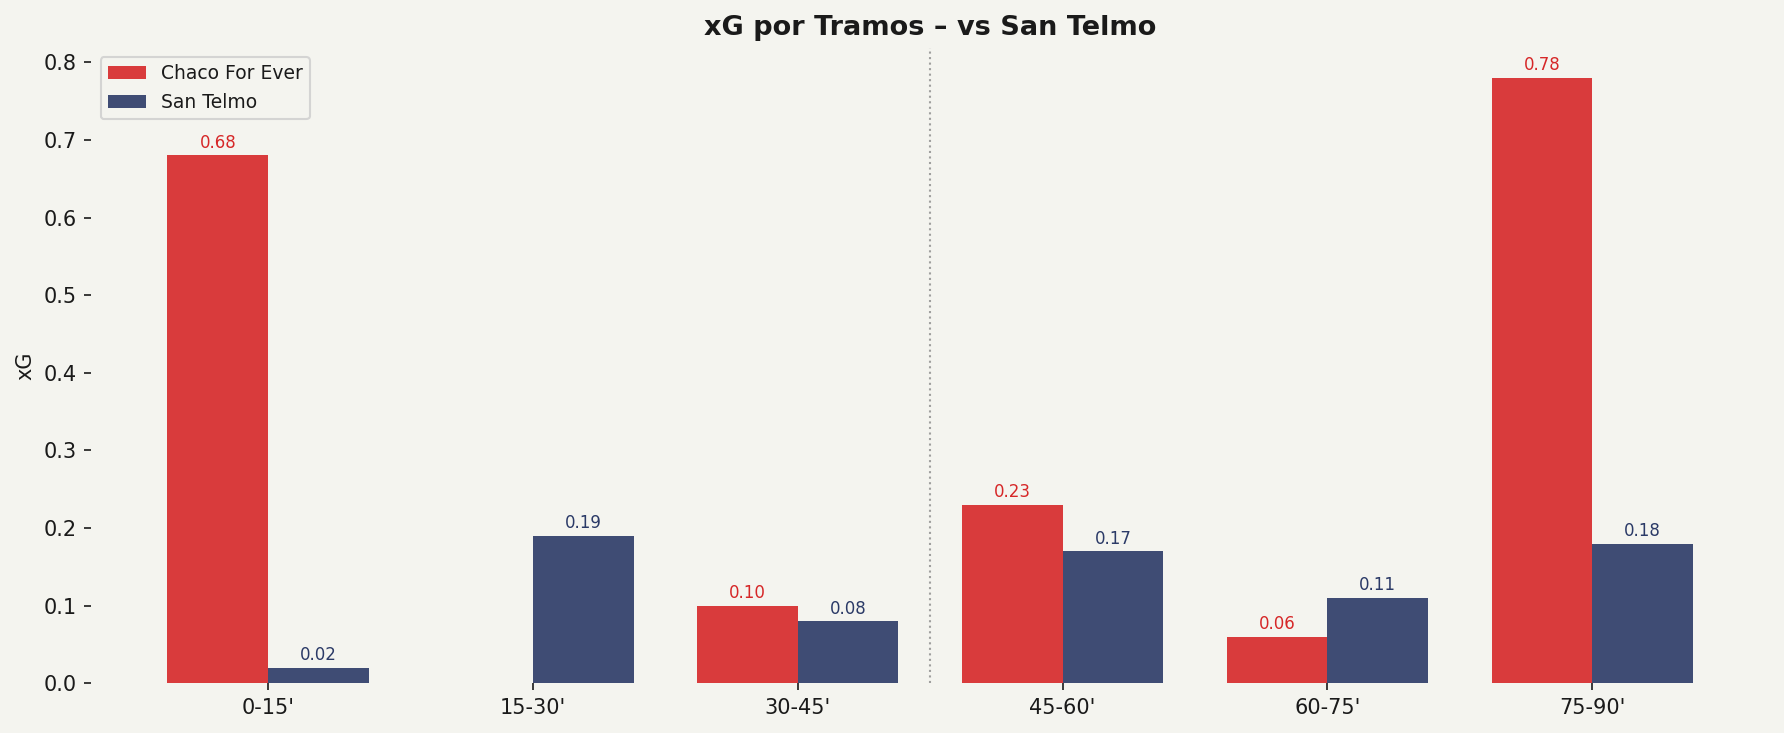
\includegraphics[width=0.98\textwidth]{xg_tramos.png}}
  \caption{El partido dividido en tramos de 15 minutos, según el peligro (xG) que generó cada equipo. Chaco (rojo) tuvo sus picos en el 0-15 ($0.68$) y en el 75-90 ($0.78$), los dos tramos de sus goles. San Telmo (azul) no superó los $0.19$ de xG en ningún tramo.}
  \label{fig:xg_tramos}
\end{figure}

% --- SECCIÓN 2: LA PREVIA FRENTE A LOS DATOS ---
\section*{2. La Previa Frente a los Datos}

\previa En el informe pre-partido marcamos tres vías para lastimar a San Telmo. Acá comparamos, sin interpretar todavía, lo que anticipamos con el dato que dejó el partido.

\subsection*{Eficacia}
\previa Predijimos que la clave era convertir: en la ida se generó mucho ($2.37$ de xG) y se empató $2$-$2$ por no definir. \textbf{Dato del partido:} $1.85$ de xG y 3 goles convertidos.

\subsection*{El penal}
\previa Marcamos que San Telmo había recibido 6 goles de penal en la temporada y que atacar el área era la vía más directa. \textbf{Dato del partido:} penal a los 89', convertido por Romero para el $3$-$1$.

\subsection*{El arquero Enrico}
\previa Señalamos que Enrico ($7.24$ de promedio en la temporada) sostenía a San Telmo casi en soledad. \textbf{Dato del partido:} 3 goles recibidos, 1 atajada y nota $6.4$.

\databox{Lo que difirió del pronóstico}{\previa Tres cosas del partido no coincidieron con lo previsto, y se dejan como dato: la posesión no fue pareja sino \textbf{68-32 para San Telmo} (esperábamos ``perfiles espejo''); la formación fue \textbf{$4$-$3$-$3$} y no el $4$-$2$-$3$-$1$ previsto; y González, el ``hombre a vigilar'', \textbf{fue suplente} (entró a los 72').}

% --- GRÁFICO 2: momentum ---
\begin{figure}[htbp]
  \centering
  \fbox{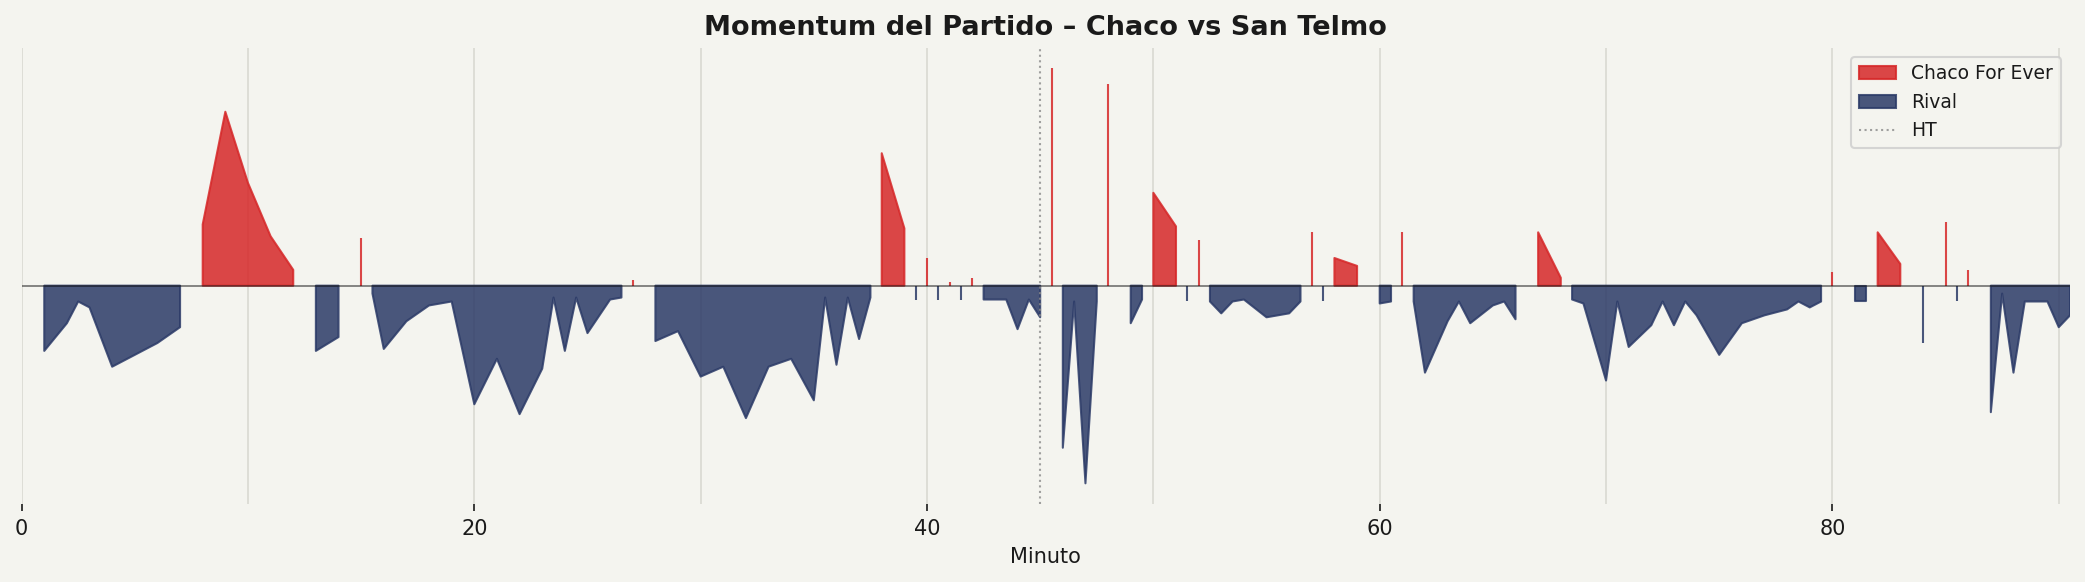
\includegraphics[width=0.98\textwidth]{momentum.png}}
  \caption{El pulso del partido minuto a minuto: en azul los avances de San Telmo, en rojo los de Chaco. El área azul es mayoritaria (San Telmo tuvo el territorio). Los picos rojos coinciden con los minutos de los goles de Chaco (8-10' y 38'). El pico azul más marcado está apenas pasado el descanso, cuando San Telmo descontó (46').}
  \label{fig:momentum}
\end{figure}

% --- SECCIÓN 3: RENDIMIENTOS INDIVIDUALES ---
\section*{3. Rendimientos Individuales}

La mejor nota del partido fue para \textbf{Matías Romero} ($9.0$): 2 goles (el del 9' y el penal del 89') y la asistencia del $2$-$0$ de Gaggi; participó en los tres goles de Chaco. Lo siguieron \textbf{Enzo Gaggi} ($7.9$, autor del $2$-$0$) y el arquero \textbf{Gastón Canuto} ($7.8$, 5 atajadas). La nota más baja fue la de J. Carrizo ($6.3$). En San Telmo, el mejor puntuado fue E. Britez ($7.4$).

\previa En la comparación de arqueros que planteaba el pre-partido (``Canuto vs Enrico''), los números del partido fueron $7.8$ y 5 atajadas para Canuto contra $6.4$ y 1 atajada para Enrico.

\temp En la fecha anterior (vs Acassuso), Romero también había sido el mejor puntuado del equipo y había convertido.

% --- GRÁFICO 3: ratings ---
\begin{figure}[htbp]
  \centering
  \fbox{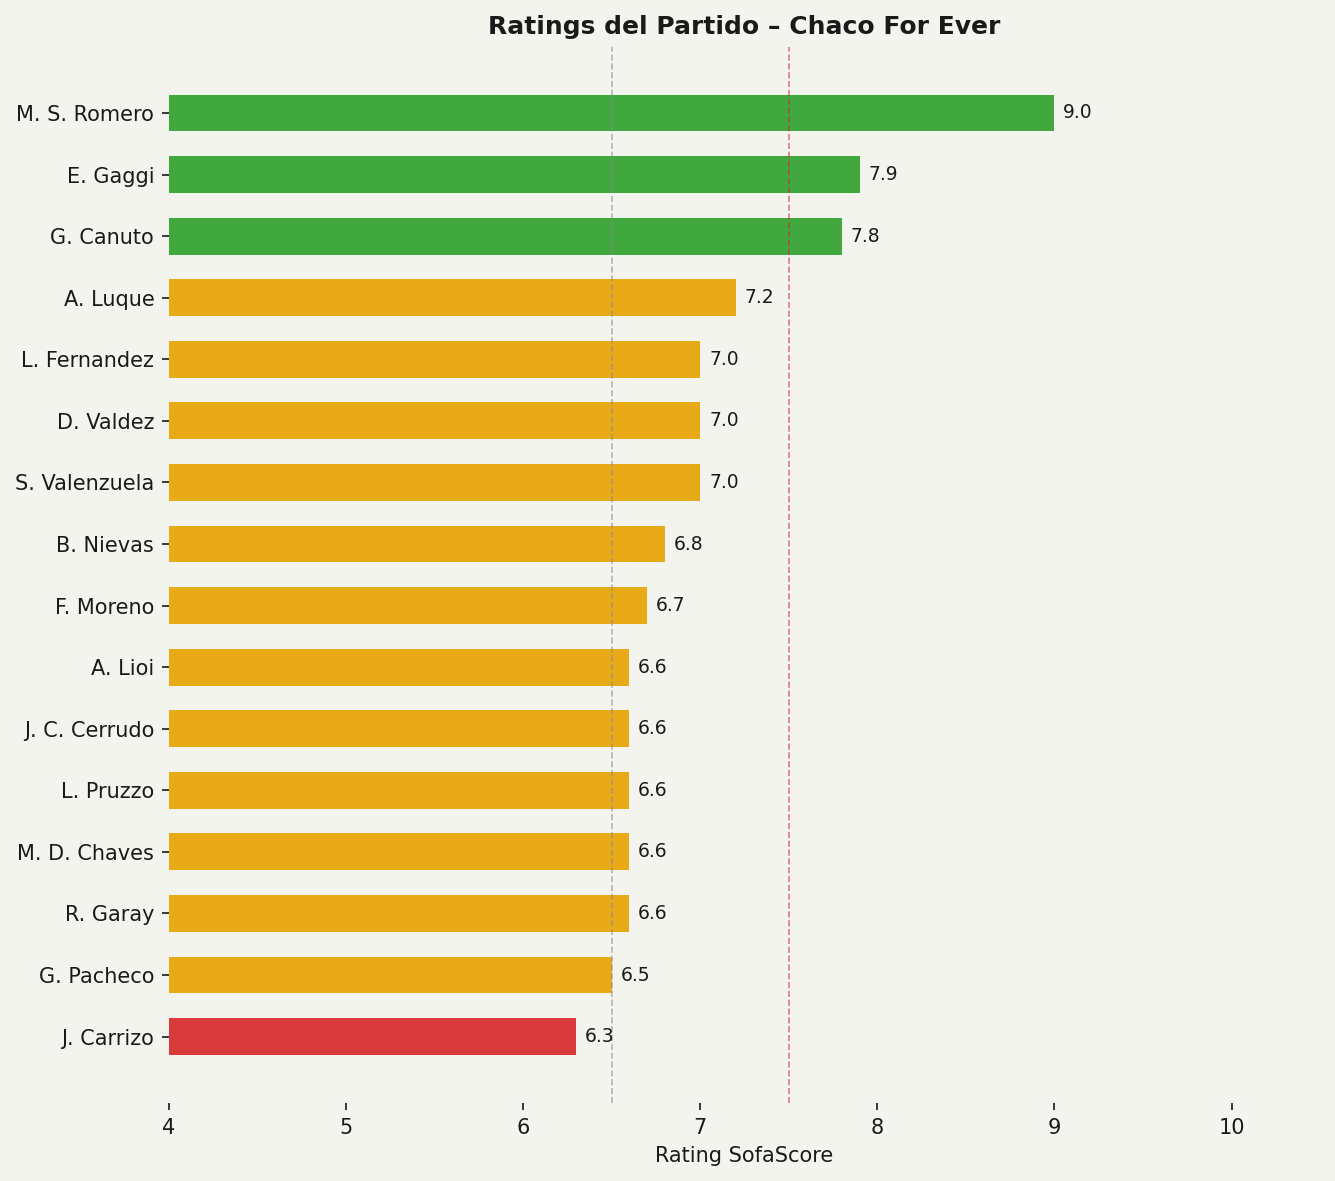
\includegraphics[width=0.90\textwidth]{ratings_jugadores.png}}
  \caption{Las notas de los jugadores de Chaco. Romero arriba con $9.0$, seguido por Gaggi ($7.9$) y Canuto ($7.8$); Carrizo, el más bajo con $6.3$.}
  \label{fig:ratings}
\end{figure}

% --- SECCIÓN 4: OTROS DATOS ---
\section*{4. Otros Datos del Partido}

\begin{itemize}
  \item \textbf{Remates de San Telmo:} 18 en total para $0.76$ de xG, de los cuales 13 fueron desde afuera del área. \previa El pre-partido preveía un ataque ``leíble'' y sin su goleador Batallini (suspendido).
  \item \textbf{Rechazos:} 46 de Chaco contra 27 de San Telmo.
  \item \textbf{xG de los goles de Chaco:} $0.61$ (Romero, 9'), $0.04$ (Gaggi, 38') y $0.76$ (Romero, penal, 89').
  \item \textbf{El gol de San Telmo:} Motroni, a los 46', con $0.04$ de xG. \temp Cae en la franja 45-60', la de más goles en contra del equipo en la temporada.
\end{itemize}

\begin{figure}[htbp]
  \centering
  \fbox{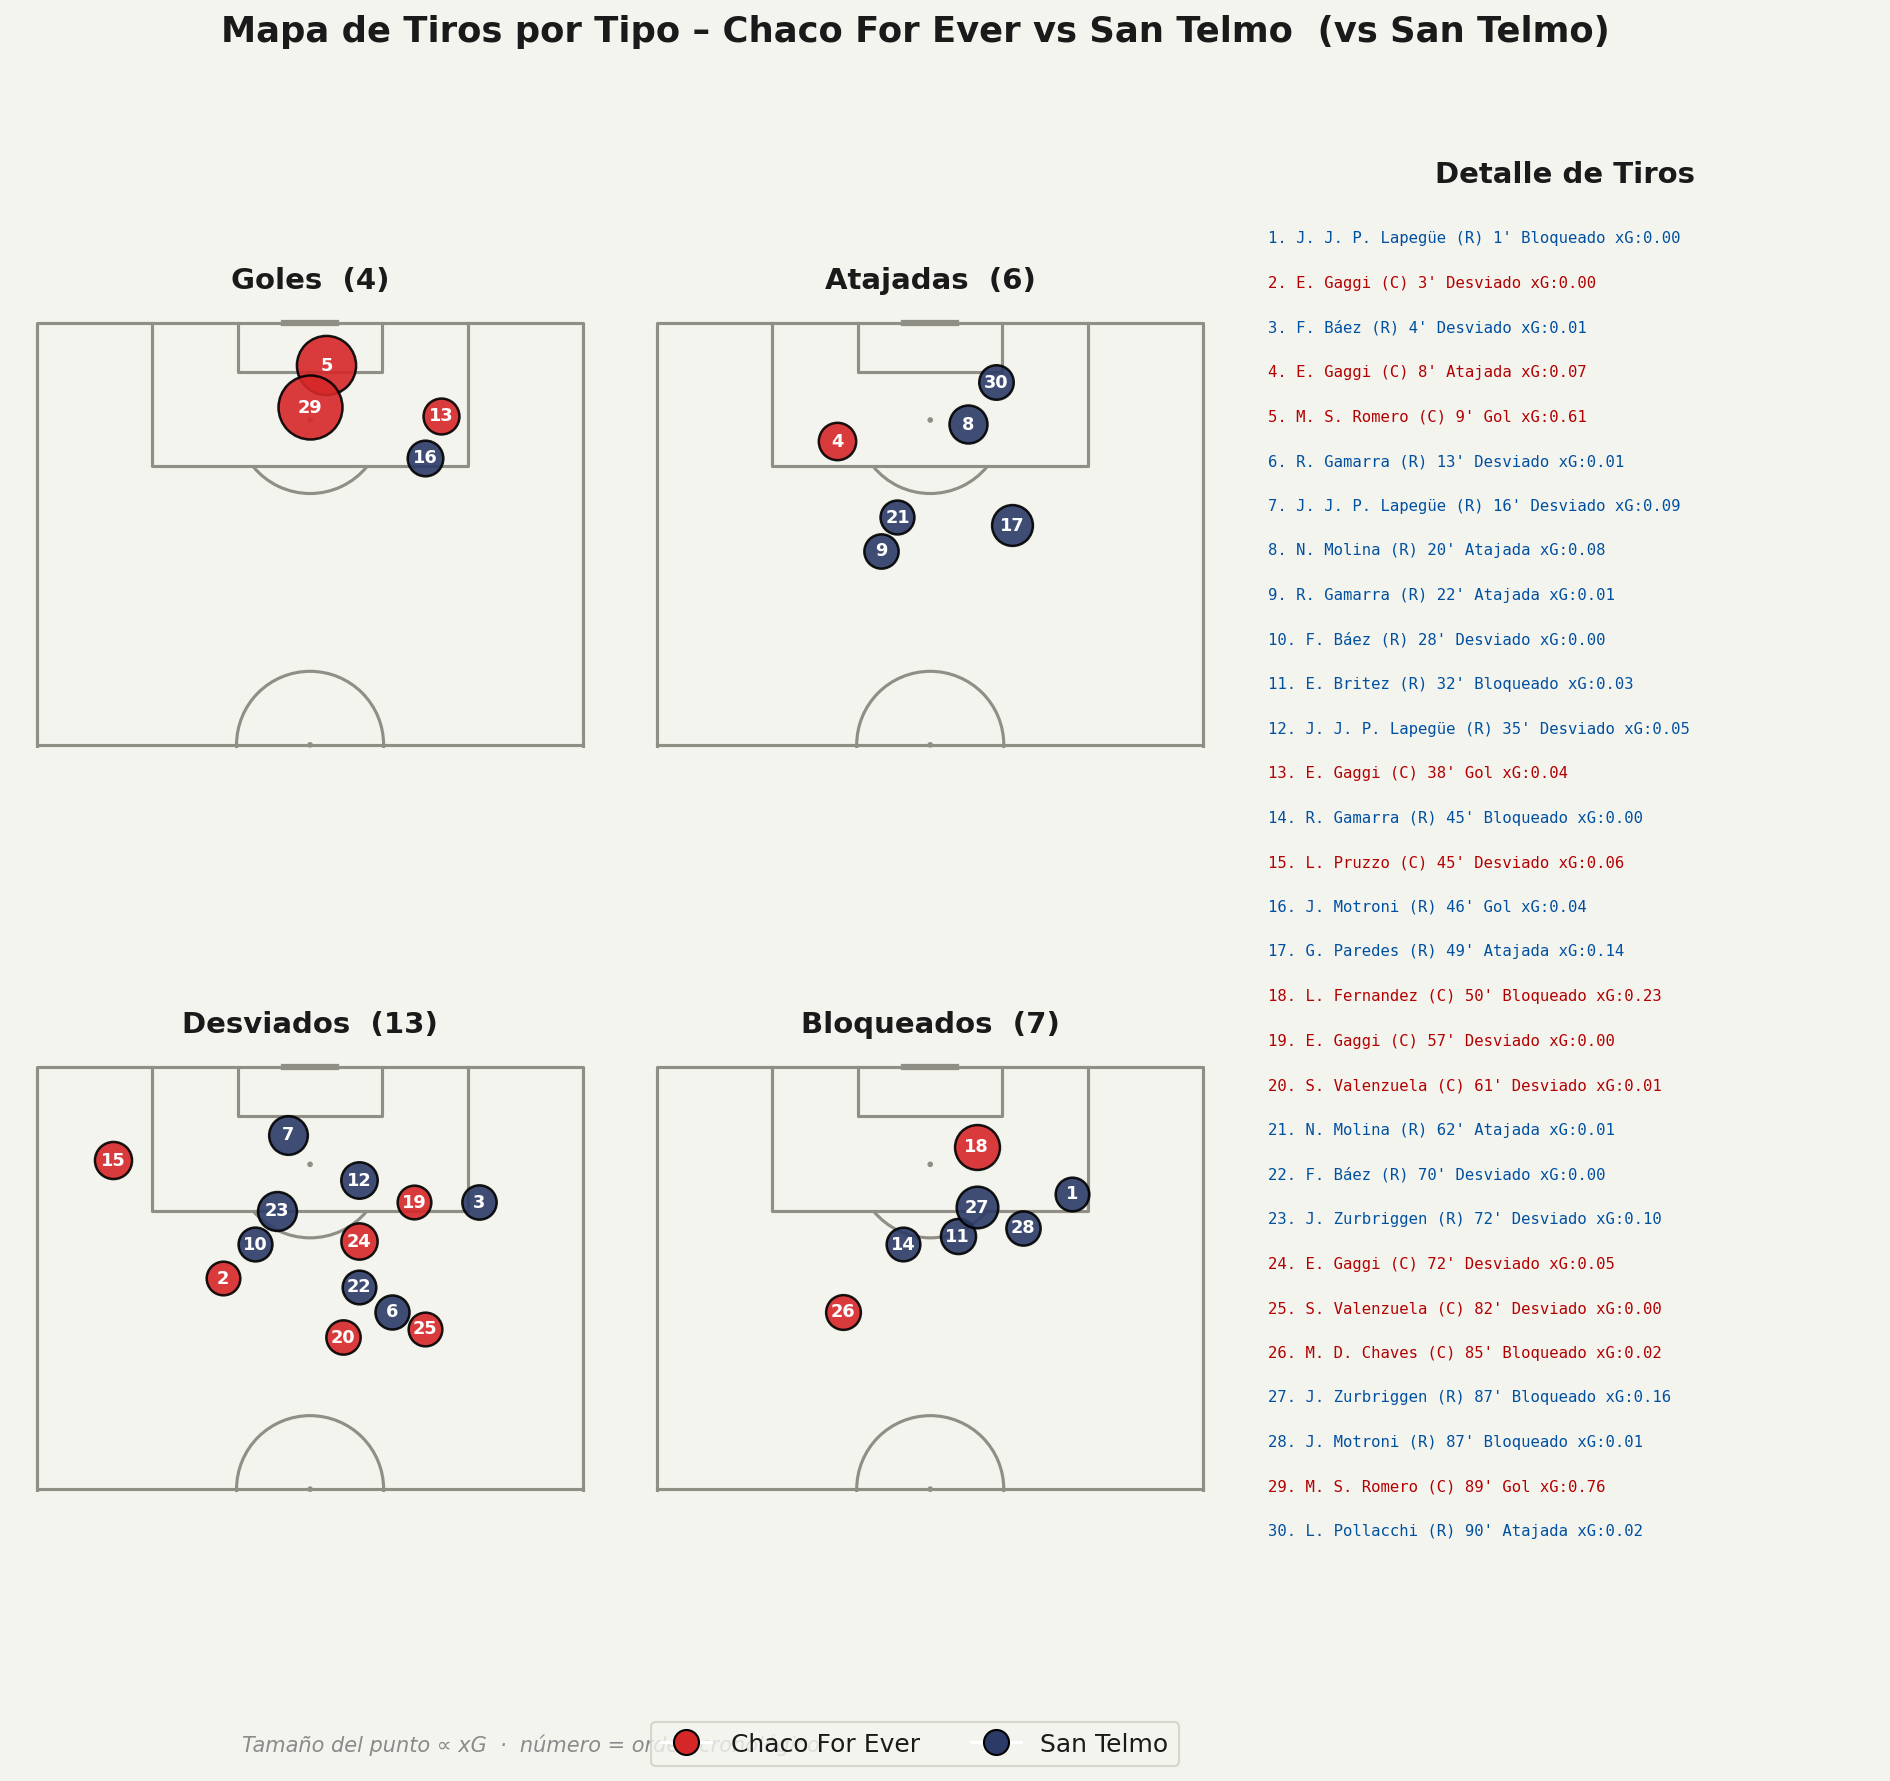
\includegraphics[width=0.98\textwidth]{shotmap_4canchas.png}}
  \caption{Todos los remates del partido, separados por tipo y con el tamaño según su xG. Los dos remates rojos más grandes son los goles de Romero, dentro del área. Los de San Telmo (azul) se concentran en ``desviados'' y ``bloqueados'', casi todos de bajo xG.}
  \label{fig:shotmap}
\end{figure}

% ==================================================================
% BLOQUE SUBJETIVO (Seccion 5): nuestra interpretacion y punto de vista
% ==================================================================

% --- SECCIÓN 5: NUESTRA LECTURA ---
\section*{5. Nuestra Lectura e Interpretación}

Hasta acá, los datos. Lo que sigue es \textbf{nuestra interpretación} de esos números y las ideas que dejamos para el cuerpo técnico.

Para nosotros fue un triunfo de eficacia y contragolpe, no de dominio. Chaco cedió la pelota (32\%) y el territorio, se replegó y lastimó en transición: generó más del doble de peligro que el rival ($1.85$ contra $0.76$) y convirtió tres. San Telmo pateó más (18 veces), pero de lejos y sin claridad; de tanto insistir le salió un solo gol. Leemos el partido como una muestra de que el equipo también puede ganar sin la pelota, un plan válido para cuando el rival propone.

\successbox{Nuestra idea central}{Apareció la eficacia que faltaba. Es el mismo equipo que en la ida generó $2.37$ de xG y no ganó; esta vez metió lo que generó, y esa fue la diferencia entre empatar y ganar. Sumado a un Canuto que sostuvo el arco cuando el partido se puso $2$-$1$, alcanzó para llevarse los tres puntos de visitante.}

\alertbox{Lo que igual nos preocupa}{El descuento llegó a los 46', apenas empezado el complemento: la misma franja en la que el equipo viene recibiendo goles toda la temporada. Esta vez no costó puntos, pero el patrón sigue ahí y es concreto para trabajar: cómo sale Chaco del vestuario en el segundo tiempo. El equipo salio igual de parado que al inicio del partido y San Telmo realido 4 cambios para intentar revertir el resultado, eso le valio un gol. Luego el equipo si se paro en un 4-4-2 mas claro.}

\subsection*{Para el cuerpo técnico}
\begin{itemize}
  \item \textbf{Se puede ganar sin la pelota.} De visitante, cediendo el balón y saliendo de contra, el equipo se llevó los tres puntos con orden. Una herramienta más para cuando el rival propone.
  \item \textbf{La eficacia es la diferencia.} Con un volumen de juego parecido al de la ida, el cambio fue definir. Sostener ese acierto es lo que separa empatar de ganar.
  \item \textbf{El arranque del complemento, otra vez.} El gol al 46' repite el patrón del año. Vale una rutina para salir metidos del vestuario y mirar esos primeros minutos en video.
  \item \textbf{Romero y Canuto, para apoyarse.} Romero encadena dos partidos siendo decisivo y le da gol y jerarquía al ataque; Canuto respondió en el momento de mayor presión.
\end{itemize}

\end{document}
